\documentclass{article}

\usepackage{amsmath}
\usepackage[final]{nips2016}
\bibliographystyle{unsrtnat}

\usepackage[utf8]{inputenc} % allow utf-8 input
\usepackage[T1]{fontenc}    % use 8-bit T1 fonts
\usepackage{hyperref}       % hyperlinks
\usepackage{url}            % simple URL typesetting
\usepackage{booktabs}       % professional-quality tables
\usepackage{amsfonts}       % blackboard math symbols
\usepackage{nicefrac}       % compact symbols for 1/2, etc.
\usepackage{microtype}      % microtypography
\usepackage{color}




%Added Apr 18
\usepackage{amsthm}
\usepackage{mathrsfs}
\usepackage[pdftex]{graphicx}
\usepackage{float}



\newtheorem{definition}{Definition}
\newtheorem{theorem}{Theorem}
\newcommand{\E}{\mathbb{E}}
\newcommand{\tvs}{\mathscr{T}}
\newcommand{\x}{\textbf{x}}
\newcommand{\y}{\textbf{y}}




\definecolor{red}{rgb}{1,0,0}
\def\red#1{{\color{red}#1}}
\definecolor{blu}{rgb}{0,0,1}
\def\blu#1{{\color{blu}#1}}

\title{Machine Learning for Stock Price Prediction}

\author{
 Juan Garcia\\
 \texttt{301281867}
 \And
 Gudbrand Tandberg \\
\texttt{83628164}
 \And
 Anson Wong\\
 \texttt{99999999}
 }

\begin{document}

\maketitle

\begin{abstract}
In this paper, we investigate the performance of machine learning models for the task of stock price prediction. After reviewing the basics of stock market prediction, we present an ensemble model that utilizes a variety of ML-techniques to forecast the future price of a given stock.
\end{abstract}

\section{Introduction}
At the heart of classical market theory lies "The Efficient Market Hypothesis", which states that markets are \emph{efficient}:

\begin{eqnarray*}
&&H_{01}: \text{A market is efficient with respect to information set $I_t$ if it is impossible}\\
&&\text{to make economic profits by trading on the basis of this information set.}
\end{eqnarray*}

A slightly stronger formulation of this hypothesis is 

\begin{eqnarray*}
&&H_{02}: \text{Stock prices are a martingale}\\
&&\text{i.e. } E\lbrack P_{t+1} \,|\, I_t\rbrack = P_t.
\end{eqnarray*}

The mere existence of profitable investment funds provide enough counter-evidence to this hypothesis to suggest the following partial refutation of the EMH: 

\begin{eqnarray*}
H_{1}: \text{there exist at least \emph{some times} where at least \emph{some part} of the market is \emph{inefficient}".}
\end{eqnarray*}

Working from this hypothesis, market investors attempt to predict markets using a combination of three broad categories of prediction methodologies: fundamental analysis, technical analysis, and data mining technologies. Fundamental analysts are concerned with the company that underlies the stock itself. Technical analysts are not concerned with any of the company's fundamentals. Instead, they seek to determine the future price of a stock based solely on the (potential) trends of the past price (a form of time series analysis). With the advent of the digital computer, stock market prediction has since moved into the technological realm, where for example internet-based data sources and machine learning algorithms are used for predicting the future. 

The stock market is essentially dynamic, non-linear, complicated, nonparametric, and chaotic in nature. The time series are multi-stationary, noisy, random, and has frequent structural breaks. In addition, stock market?s movements are affected by many macro-economical factors such as political events, firms' policies, general economic conditions, commodity price index, bank rate, bank exchange rate, investors' expectations, institutional investors? choices, movements of other stock market, psychology of investors, etc. It is our belief that the only reasonable way of overcoming all these difficulties is by harnessing the power of big data and modern machine learning algorithms and architectures. Perhaps even it is possible to devise models of stock prediction that will allow fully automated investment funds to operate with a higher success than funds reliant on human "expert knowledge".

\blu{You should explicitly state your contribution in the introduction of the paper,}

\section{Related Work}

This is a citation \cite{vapnik1999overview}.

\section{The Data}
\subsection{Data Cleaning}
\subsection{Feature Engineering}

\section{Our Model}
\subsection{SVM Regression}
\subsection{Gaussian Processes}
In this section we are going to start with a brief introduction to Gaussian Processes, what they are
and how to use them in calculations. Let us begin with a formal definition


\subsubsection*{Introduction}
\begin{definition}\label{dfnGP}
A Gaussian process (GP) is a collection of random variables $\{g(x)\}_{x\in A}$, for some set $A$, 
possibly uncountable,
 such that any finite subset of random variables
 $\{g(x_{k})\}_{k=1}^{N}\subset\{g(x)\}_{x\in A}$ for 
$\{x_{k}\}_{k=1}^{N}\subset A$ are jointly Gaussian
\cite{rasmussen2006gaussian}. 
\end{definition}

A GP is specified by a mean function and a covariance operator or kernel. 
Following  Rasmussen \cite{rasmussen2006gaussian} we define
\begin{eqnarray*}
m(x):=\E(g(x)),\qquad\text{(Mean)}\\
k(x,x'):=\E((g(x)-m(x))(g(x')-m(x')))\qquad\text{(Kernel)}.
\end{eqnarray*}
If $\{g(x)\}_{x\in A}$ is a GP with mean $m(x)$ and covariance $k(x,x')$ we will write
\begin{equation*}
g(x)\sim \textbf{GP}(m(x),k(x,x')).
\end{equation*} 

For a fixed $x\in A$, a realization of the  random variable $g(x)$ represents
a possible value of a function $M(x)$ we want to approxiamte. 
The mean function at that point $x$, i.e. $m(x)$ 
represents the best prediction about the true value of $M(x)$. Later we will show that the uncertainty 
associated to that prediction is given by the quantity $k(x,x)$.
\newline

The reason why the definition of a  Gaussian processes is useful in practice is that  GPs are 
completely characterized by $m(x)$ and $k(x,x')$\cite{lifshits2012lectures}. 
 For example a  common covariance or kernel is the
 squared exponential (SE) function
\begin{equation}\label{eqnsquareexponential}
k(x,x')=e^{-\frac{1}{2}\|x-x'\|_{2}^{2}}.
\end{equation}
The reason to use the name squared exponential instead of Gaussian is to avoid confusion with
the probability distribution.
This  covariance function tells us that points that are close to each other
are highly correlated whereas far away points have a correlation that decays exponentially fast.
There are some `standard' ways to choose the covariance function depending on the kind
of regularity we want for the realizations of the GP.
Some of the most common kernels are \cite{rasmussen2006gaussian} (setting $r=\|x-x'\|_{2}$)

\begin{itemize}
\item Squared-Exponential: $k(r;\theta)=e^{-\frac{1}{2}(\frac{r}{\theta})^{2}}$
\item Exponential: $k(r;\theta)=e^{-\frac{r}{\theta}}$\\
\item Matern $\frac{3}{2}: k(r;\theta)=(1+\frac{\sqrt{3}r}{\theta})e^{-\frac{\sqrt{3}r}{\theta}}$.
\item Matern $\frac{5}{2}: k(r;\theta)=(1+\frac{\sqrt{5}r}{\theta}+\frac{5}{3}
(\frac{r}{\theta})^{2})e^{-\frac{\sqrt{5}r}{\theta}}$.
\item Power-Exponential: $k(r;\theta,p)=e^{-(\frac{r}{\theta})^{p}}$.
\end{itemize}

Mathematically, GPs are measures on function spaces. We now discuss them in this
context following \cite{lifshits2012lectures}.




\subsubsection{Distributions Over Function Spaces}
Interesting function spaces (e.g. $L^{p}$ spaces, Sobolev spaces, etc...) are 
normed vector spaces, with a topology inherited from the metric induced by the norm, and so 
, function spaces are topological vector spaces (TVS). 

Let $\mathscr{T}$ be a TVS and  let $\mathscr{T}^{*}$ be its topological dual. 
We will denote the action of an 
element $h\in\tvs^{*}$ over an element $z\in\tvs$ with $\langle h,z\rangle$. Moreover 
we  define a random variable taking values in $\tvs$ as a map 
\begin{equation*}
X:(\Omega,\mathscr{F},P)\longrightarrow\tvs,
\end{equation*}
that is measurable with respect to the $\sigma$-algebra generated by the topology
of $\tvs$. This $\sigma$-algebra is known as the Borel $\sigma$-algebra for $\tvs$.
The triple $(\Omega,\mathscr{F},P)$ is a probability space. 
We use the shorthand notation  $X\in\tvs$ whenever the random variable $X$ takes vales in $\tvs$. 
For example if $\tvs=L^{2}(\mathbb{R})$,  then  $X\in L^{2}(\mathbb{R})$ means that $X$ is a measurable
map from the probability space $(\Omega,\mathscr{F},P)$ into $L^{2}(\mathbb{R})$.

We say that a random variable $X\in\tvs$ is called Gaussian if $\langle h,X\rangle$ is
a Gaussian random variable on the real line for all $h\in\tvs^{*}$. We say that an element $a\in\tvs$ is the 
expectation of $X\in\tvs$ if 
\begin{equation*}
\E(f,X)=\langle f, a\rangle,\qquad\text{for all }f\in\tvs^{*}.
\end{equation*}
Also a linear and positive definite operator $K:\tvs^{*}\longrightarrow \tvs$ 
is called the covariance operator (e.g. covariance
matrix in the finite dimensional case) if
\begin{equation*}
cov(\langle f_{1},X\rangle,\langle f_{2},X\rangle)=\langle f_{1},Kf_{2}\rangle,
\end{equation*}
for all $f_{1},f_{2}\in\tvs^{*}$. In this case we say that $X$ is distributed as 
$\mathcal{N}(a,K)$ if  $X$ is Gaussian with mean $a$ and covariance operator $K$. It is worth mentioning
that given a covariance operator $L$ and an element $b\in\tvs$ the distribution $\mathcal{N}(b,L)$
does not always exist. But if it does exist, to define the  Gaussian measure $\mathcal{N}(a,K)$, it is
only necessary to know $a$ and $K$.
\newline

As an example consider the  $\tvs=\mathbb{C}(T)$ where 
$T\subset\mathbb{R}^{n}$ and $T$ is compact. This is the  space of real valued continuous functions 
defined in 
$T$. This  is a Banach
space with the norm \cite{bressan1900lecture}
\begin{equation*}
\|h\|=\max_{x\in T}|h(x)|.
\end{equation*}
The dual space of $\tvs$ is given by $\tvs^{*}=\mathbb{M}(T)$ the set of signed measures defined on 
the Borel $\sigma-$ algebra of  $T$. In this 
case the duality pairing is given by 
\begin{equation*}
\langle\mu,g \rangle=\int_{T}gd\mu.
\end{equation*}
Given a GP,  $\{g(t)\}_{t\in T}$ (see definition \ref{dfnGP}) with mean function $m(t)$ and 
covariance kernel $k(t,t')$, it can be thought as a Gaussian measure $\mathcal{N}(m,K)$
where
\cite{lifshits2012lectures} 
\begin{eqnarray*}
\E(f)=m\in\mathbb{C}(T), \\
(K\nu)(t)=\int_{T}k(t,t')\nu(dt'),\qquad\text{for }\nu\in\mathbb{M}(T).
\end{eqnarray*}

The above example shows the connection between GPs and distribution over function spaces. More
precisely how it is connected to Gaussian measures in function spaces. Now we move on
into explaining how to use GPs in a practical setting.

Assume  we have some  results  (training inputs) from a function $M(\cdot)$ we want to approximate,
$\{(\textbf{x}_{i},y_{i})\}_{i=1}^{m}\subset\mathbb{R}^{n}\times\mathbb{R}$, where $M(\textbf{x}_{i})=y_{i}$. For
simplicity we assume no trend in the training inputs. Given this data 
we would like to infer  possible values of $M(\cdot)$ on another set of points 
$\{\textbf{x}_{j}^{*}\}_{j=1}^{k}$ (test inputs). The way to do this is as follows: consider the $GP$, $\{f(\x)\}_{\x\in A}$
where $A$ is given by the training and test inputs. Then we create the random vectors
\begin{eqnarray*}
\textbf{f}=\begin{bmatrix}f(\textbf{x}_{1}) & \ldots & f(\textbf{x}_{m}) \end{bmatrix}^{T}, \\
\textbf{f}^{*}=\begin{bmatrix}f(\textbf{x}_{1}^{*}) & \ldots & f(\textbf{x}_{l}^{*}) \end{bmatrix}^{T},
\end{eqnarray*}
according to the definition of a GP, these vectors are  jointly Gaussian, i.e. 
\begin{equation}\label{eqnconditional}
\begin{bmatrix}
\textbf{f} \\
\textbf{f}^{*}
\end{bmatrix}\sim\mathscr{N}\left(0,\begin{bmatrix} K(X,X) & K(X,X^{*}) \\
						    K(X^{*},X) & K(X^{*},X^{*}) \end{bmatrix}
\right),
\end{equation}	
The zero mean models the assumption of no trend in the data. 
Here
$(K(X,X))_{ij}=cov(f(\x_{i}),f(\x_{j})), K(X,X^{*})_{ij}=cov(f(\textbf{x}_{i}),f(\x_{j}^{*}))$ and so on.

In this work we are assuming that the realization of the vector $\textbf{f}$ is known (this vector could be
the known prices of a particular stock at different times).
We want to make inferences about the vector $\textbf{f}_{*}$ (This vector represents the prediction of  future values
 of the stock under study, for example),
therefore we are looking for the distribution of $\textbf{f}_{*}|\textbf{f}$. By well known properties
of the multivariate Gaussian distribution we  obtain  \cite{lifshits2013gaussian}
\begin{equation}\label{eqnformulameancovariance}
\textbf{f}^{*}|\textbf{f}\sim\mathscr{N}\left(K(X^{*},X)K(X,X)^{-1}\textbf{f},
K(X^{*},X^{*})-K(X^{*},X)K(X,X)^{-1}K(X,X^{*})\right).
\end{equation}
Note that in the mean $K(X^{*},X)K(X,X)^{-1}\textbf{f}$ if we replace the test inputs in the matrix
$K(X^{*},X)$ by the train inputs, then, this matrix transforms into $K(X,X)$. With this, the mean
would be $K(X,X)^{-1}K(X,X)\textbf{f}=\textbf{f}$ and the covariance matrix would be the zero matrix. 
In this case the predicted values by the distribution are exactly the training inputs $\textbf{f}$.
This shows that the mean of the distribution interpolates the values  of whatever function we are trying to 
approximate. The prediction for
the output of 
a point $\textbf{x}^{*}$ that is not part of the training set lives, with $68\%$ of confidence, in the interval
\begin{equation*}
K(\textbf{x}^{*},X)K(X,X)^{-1}\textbf{f}\pm K(\textbf{x}^{*},\textbf{x}^{*})-
K(\textbf{x}^{*},X)K(X,X)^{-1}K(X,\textbf{x}^{*}).
\end{equation*}

This shows that choosing the covariance kernel 
is a crucial step in the fitting process. In practice we choose from a standard collection of kernels
that give us different degrees of flexibility for the GP. Among these standard kernels we have: Gauss,
exponential, Matern $\frac{3}{2}$ and $\frac{5}{2}$ and power-exponential.

Covariance kernels are usually defined in terms of parameters, so depending on the data 
we can find the parameters that best suit the data. Given a kernel class, the question now is: how
to choose the right parameters for the data? One possibility is by optimizing the likelihood, given by
\begin{equation*}
p(y^{*}|\{(\x_{i},y_{i})\}_{i=1}^{m},\theta).
\end{equation*}
By definition \ref{dfnGP} we know that the conditional probability has to be distributed as
a multivariate normal distribution. More precisely

\begin{equation}\label{eqnlikelihoodExponential}
p(y^{*}|\{(\x_{i},y_{i})\}_{i=1}^{m},\theta)=\frac{1}{(2\pi)^{\frac{m}{2}}det(K_{y^{*}}(\theta))^{\frac{1}{2}}}
e^{-\frac{1}{2}(y^{*T}K_{y^{*}}(\theta)^{-1}y^{*})}.
\end{equation}
Where $K_{y^{*}}(\theta)$ is the matrix $K(X,X)$ in equation (\ref{eqnconditional}). We explicitly
show the dependence on $y^{*}$ and $\theta$ for clarity. We want to maximize (\ref{eqnlikelihoodExponential})
with respect to $\theta$.
This goal is unchanged if we take logarithms on both sides and minimize the negative
of this function  the equation to get\footnote{The reason to do this is because most
software packages for optimization, search for the minimum not the maximum.}


\begin{equation}\label{eqnloglikelihood}
-\log(p(y^{*}|\{(x_{i},y_{i})\}_{i=1}^{n},\theta))=\frac{1}{2}y^{*T}K_{y^{*}}(\theta)^{-1}y^{*}+
\frac{1}{2}\log|K_{y^{*}}(\theta)|+\frac{n}{2}\log(2\pi).
\end{equation}

By minimizing this equation with respect to $\theta$ we find a possible value of this parameter
that explains the best the data $y^{*}$ given $(\x_{i},y_{i})$.

\subsubsection*{GPs for Stock Market Prediction}
In this work we have data from 6328 stocks and for each stock we have 504 days of data of closing price, open price,
Volume of trading, daily high price and daily low price. To test GPs for stock market prediction we are going
to try to predict the closing price for every stock we have data of. To be more precise, let us start with an 
example.  Consider the following data of the close price for a stock price XXX (names of the stocks?)

\begin{figure}[H]
\centering
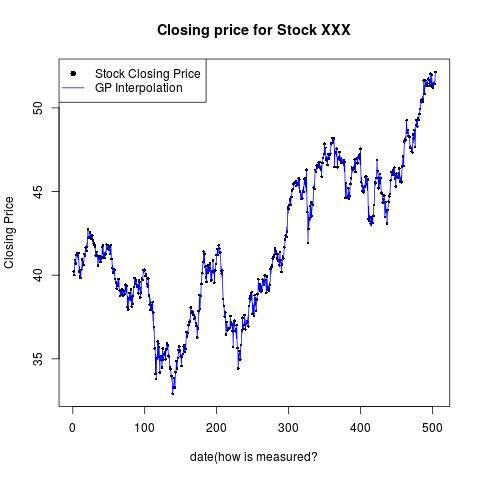
\includegraphics[scale=0.4]{../Algorithms/Juan/figures/GPFitExample}
\caption{GPfitExample}
\end{figure}

In this case we used as a covariance function an exponential kernel of the form
\begin{equation}\label{eqnkernel}
k(t,t';\theta)=\exp\left(\frac{|t-t'|}{\theta}\right),
\end{equation}
where the value of $\theta$ is 6.07. This value was found using MLE. The reason to choose this kernel 
is because we know that the function to be approximated is continuous but not differentiable and
the kernel in equation (\ref{eqnkernel}) gives samples with this property. 
\textbf{Talk a little bit more about how this kernel is an acceptable choice}

\subsubsection*{GP for prediction}
By looking at the performance in the interpolation of the GP, it is natural to ask how
is the performance of the GP when it comes to prediction. To assess the quality of the prediction
of the GP we analyse the 6328 stocks and predict the closing price of each stock from one to seven days
in the future. Then we calculate the proportion of success in the prediction. It is necessary to take
into account that we are just testing the $GP$ in terms of its ability to predict if the stock
will go up or down, not how close to the actual price it is. The results obtained are shown below

\begin{figure}[H]
\centering
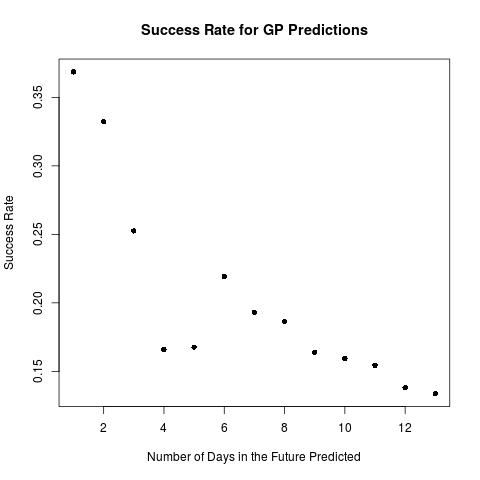
\includegraphics[scale=0.4]{../Algorithms/Juan/figures/successPlot}
\caption{Success of the GP}
\end{figure}

It is interesting to notice that the further away in the future we are trying to do a prediction
the worst the prediction it is. This is not what we expected since having a very bad accuracy rate
means some kind of predicting capabilities. To understand why, consider the case where the prediction
is wrong a 100\% of the times. In this case if we always act contrary to the prediction then we will
have a 100\% success rate in predicting if an stock goes up or down. The fact that the GP is getting
worst at predicting is something that needs to be understood. This is going to be our next task

\subsubsection{Why GPs are so Terrible (Good?) at Predicting?}
To understand what is going on consider the following sequence of plots
were we use GPs to predict the outcome of the closing price of the stock XXX

\begin{figure}[H]
\centering
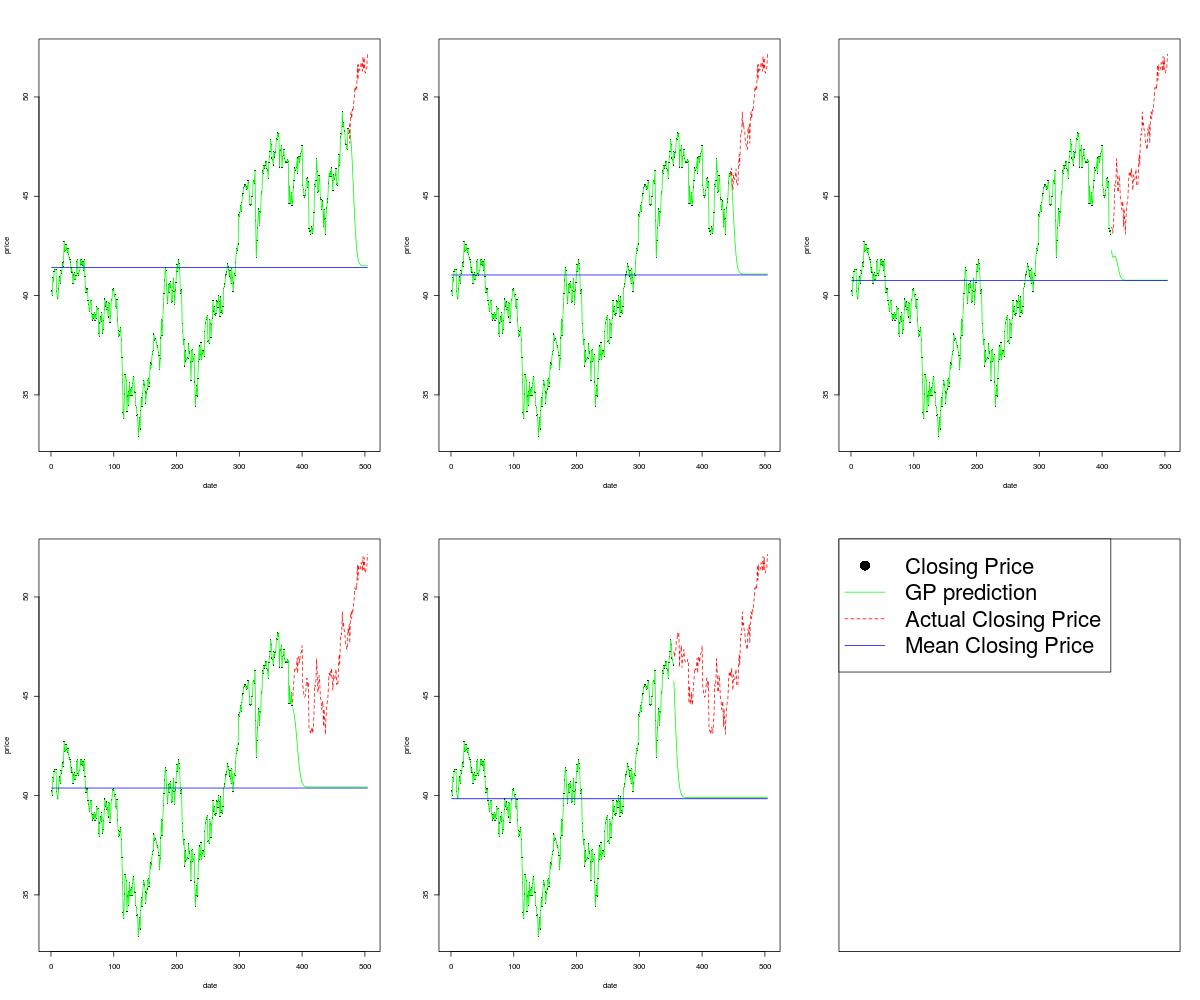
\includegraphics[scale=0.35]{../Algorithms/Juan/figures/snapshots}
\caption{Snapshots of the prediction}
\end{figure}

This results shows that when considering the past history of every stock isolated to predict its future, is
not possible. In this case we can see that the prediction of the GP converges to the mean value
of the closing price. \textbf{Can we talk about the following theorem?}

\begin{theorem}
Given a set of training points $(\x_{i},y_{i})_{i=1}^{n}$ and  a GP with a covariance kernel of the form 
$k(\|\x-\x'\|;\theta)$ and mean $m(\x)$ then 
under some suitable conditions we have 
\begin{equation*}
\lim_{\|\x\|\rightarrow\infty}m(\x)=\frac{1}{n}\sum_{i=1}^{n}y_{i}.
\end{equation*}
\end{theorem}




\subsection{Markov Model}
\subsection{...}
\subsection{The Ensemble Learner}

\section{Results}

\section{Discussion}
\blu{State the main conclusions that are obtained from this course project.
List at least one strength and one weakness of your contribution. Briefly state what you would do with
more time}

\bibliography{bibliography} 

\end{document}
